\documentclass{article}
\usepackage{graphicx} % Required for inserting images
\usepackage{amsmath}
\usepackage[utf8]{inputenc} % For input encoding
\usepackage{geometry} % For page margins
\geometry{a4paper, margin=1in} % Set paper size and margins
\usepackage{titlesec} % For section title formatting
\usepackage{enumitem} % For itemized list formatting
\usepackage{hyperref} % For hyperlinks
\usepackage{pgfplots}


\title{Honors Econ}
\author{Anthony Yoon}
\date{September 2024}

\begin{document}

\maketitle
\tableofcontents


\begin{abstract}
    These are my notes for the Elements of Economic Analysis Honors. The first quarter is taught by Professor Lima so the first third of these notes will be dedicated to the quarter of that. For any legal reasons, I am not trying to replicated Lima's notes in any fashion whatsoever. 
\end{abstract}

\section{Lecture 1: Laying the foundation}
\subsection{Covering of the class structure}
The first half of this class was dedicated towards the covering of the syllabus and other materials. He recommended to read 
\begin{itemize}
    \item Perloff
    \item Varian (Less math-y)
    \item Besenko and Braevitgan (Spelling on the last one is not sure)
    \item Kreps
    \item Jehle - Reny 
    \item Mas - Castell (Not sure about the spelling on this one), Whinston, Greene
\end{itemize}
\subsection{The actual meat of this lecture}
\subsubsection{The motivation and creation of economics}
This class is dedicated to what we call the \textbf{\textit{economical approach}}. This approach was mainly derived by Gary Beckerr's paper \textit{The Economical Approach to Human Behavior}. This class is also dictated by the paper \textit{Methodology of Positive Economics} by Milton Friedman. These 2 papers are papers that you apparently have to read so, get to reading if you haven't. \\


The reason why these papers are so highly valued by Lima is the fact that these papers lay the scientific foundations for economics as a field. These include science philosophy and methodology. If we were to examine how knowledge in colleges were divided up, these include the different departments that are in play. We have the broad departments like the Physical Sciences Department and the Social Sciences Department, and inside these departments we have more specialized departments like the Economics Department, Psychology Department, and so forth. Most of these mini departments can be considered to be centered around a question that people are interested in. I'm sure we can make something up for each respective department, but the general idea is there. And in doing so, we essentially segregated these disciplines into many different ones. The reason why these two papers are so important are because of how they promoted cross discipline studies or other things. As we can see: \footnote{My own written notes are not so clear here, so I will update once I read these papers}. 
\begin{itemize}
    \item Becker: Economists live in discrimination and have something to say about that, so Becker essentially invaded sociology. 
    \item Friedman: He also invaded something, but I don't know what. I didn't write it down.
\end{itemize}
Here we will outline the approach that Becker outlined in his paper, in this class we were only able to outline 2 out of the 5. But one thing to note is that \textbf{because of the assumptions that we make in economics, every model that we make is going to be incorrect.} It is very hard to outline every single possibility and occurrence in the real world so every model is not accurate.\\
\subsubsection{The first assumption}
\begin{center}
    \Large \textbf{\emph{Resources are scarce}}
\end{center}
A logical way of thinking about this is to examine time itself. Within each moment of time, there are only a finite number of things that we can do. We can only pack each minute with so many things. \\


However, how does this manifest itself mathematically? This phenomenon is what we call \textbf{constraints}. There are two types of constraints that we study \textbf{Explicit} and \textbf{Implicit} constraints. In this course, we mainly focus on explicit constraints, but the main differences between these types of constraints are:
\begin{itemize}
    \item Explicit: We have an explicit limit. This could mean that a credit card has hard limit of some amount or an individual only has 50 US Dollars.
    \item Implicit: These are things that are implicit. Some might call them unwritten rules so to speak.
\end{itemize}
Both of these can be addressed using a model, which may be in the form of an inequality or an equation. There are many types of constraints that we can talk about. The first one that we can talk about are \textbf{budget constraints}.\\


\textbf{Budget Constraints} are usually denoted by the symbol $m$.  We can of this in this sense: if we have a set budget $m$, and we were only interested in one item, we would could just burn all the money on that one good. However, when we consider other options, then our money gets sparse. Thus, we can get something in this form 
\[
\begin{array}{ccc}
    \text{Command of resources} & \hspace{1pt} & \text{Expenditure} \\
    m & \geq & p_x x + p_y y
\end{array}
\]
where x and y can be anything you want. The reason why the greater than or equal to sign is that we cannot exceed a certain amount. $x$ and $y$ stand for anything you want, whether that be apples and oranges, market prices, and so forth. Note that in this class, we mostly are determining market prices. So, we can say that $x$ and $y$ are units of good x and y respectively. These goods also have to be \textit{continuous} because we need to apply calculus to these variables. $p_x$ and $p_y$ stand for price per unit $x$ and $y$ respectively. Note that these prices are \textit{ratios} and hence rates we can use to (I assume) exploit calculus with. However, logicaly we need to have a positive number of goods, so we can say that 
\[
x \geq 0 \hspace{1cm} y \geq 0
\]
So in total we have the following expression. 
\[
\begin{array}{ccc}
     \text{Command of resources} & \hspace{1pt}  & \text{Expenditure} \\
     m & \geq & p_x x + p_y y\\
     \text{Constraint:} & x \geq 0 & y \geq 0\\ 
\end{array}
\]
This is called a \textbf{budget set}. An ordered pair of (x,y) would be called a \textbf{bundle}. However, having doing some amount of calculations and some reductions, we eventually can reach a \textbf{budget constraint}, which is denoted as follows:
\[
p_x x + p_y y = m
\]
where we can think that of a person that spends all of their money. Now we have to note that this is a single period problem, where we can only know what is going on in one point in time. Note that the budget set is also called the \textbf{canonical constraint} at times and is the main thing that we want to simplify to.\\


Another type of constraint is the \textbf{time constraint}. After all, there is only a finite amount of time, where 
\[
t_1 + t_2 + t_3 +  \dots + t_N = T
\]
where $t$ is an event and $T$ is the total amount of time, or time endowment. We can see this in the following example, when it comes to labor markets. \\


Let $L$ and $R$ mean the time spent on labor and rest respectively. Therefore, we can set the following:
\[
L + R = T
\]
\textit{Note}: All time must be accounted for, no time should be left out, even if you die, the time you die will be considered time spent dead and will be accounted for. And from here, we can see how the money that the worker makes can equal the actual budget constraint, as denoted here:
\[
wL = pC
\]
where $w$ are the wages and $L$ are the hours worked, and $p$ is the cost of wanted items and $C$ is the number of things that a person wants. A remark was made around here, economics is a powerful tool as we can generalize it for all situations. We can say that we have one theory for why we behave  in the labor market and the supermarket. Additionally, there is another idea that substitution is key in economics here. we can see that 
\[
L + R = T 
\]
\[
L = T - R
\]
substituting the above equation yields 
\[
pC = w(T - R)
\]
\[
pc + wR = wT
\]
where $wT$ is the full income that one makes, where the full 24 hours are worked. Note that the above equation is in the same form of the canonical form, a testament to the simplification methodology. There are also many other constraints, such as the biological constraint, where the number of kids that are physically possible are limited. Another idea of a constraint is supply and demand. This is seen as 
\[
D \leq S
\]
where demand cannot succeed supply. If it does, then the resource becomes not scarce and and the good becomes 0. \footnote{Not sure about this check.} Note that all constraints will have some sort of a negative slope, where it can be seen here:
\begin{center}
    \begin{tikzpicture}
    \begin{axis}[
        axis lines = left,
        xmin=0, xmax=1,
        ymin=0, ymax=1,
        xlabel= product x,
        ylabel= product y,
        domain=0:1
    ]
    % Plot the line y = -x + 1
    \addplot[color=blue, thick] {-x + 1};
    \end{axis}
\end{tikzpicture}
\end{center}
Where the X and Y intercepts are $\frac{m}{p_x}$ and $\frac{m}{p_y}$ and the slope is $\frac{-p_x}{p_y}$
\subsubsection{The 2nd approach}
The 2nd approach is \textit{Preferences are stable}. Lima went on a massive rant about this, but the gist of the rant is that \textit{we need to make sure that when a preference changes, then that change directly causes something}. He attributed this to something along the lines of "If I pull a lever, then that causes a change". However, this assumption is actually considered controversial. But ignoring that \footnote{I am not going to go into this so I don't really care about this lmao}, another reason why we make this assumption is that determining what makes a change in preference is hard, and thus assuming a stable preference is an economically good assumption. And thus, in making this assumption, preference is playing a causal role in changes in behavior. \\

\noindent
There are two types of preference change: \textbf{Exogenous} and \textbf{Endogenous}. They are as follows:
\begin{itemize}
    \item \textbf{Exogenous}: Caused by external changes. I think this is like there are no oranges at the supermarket but double check. \textbf{Check for clarification here}
    \item \textbf{Endogenous}: This are caused by internal changes, these can be advertising and rational addiction. An example of rational addiction would be that I ate too much chocolate yesterday, and I will not eat it today. At least in this change of preference, we are linking past consumption to current consumption.
\end{itemize}
An example of this is that children became more expensive during the industrial revolution because originally children were working on the farms. But, a tractor is arguably cheaper than 10 children working on a farm, so other opportunities had to be focused for the children, which thus raised costs of raising children. Thus, this is a change in a preference as we want to have less children during the industrial revolution. But, in this class we always assume that \textbf{Preferences will never change}
\subsubsection{Key Takeaways}
Key takeaways from this lecture. 
\begin{itemize}
    \item The paper \textit{The economical approach to human behavior} by Gary Beckker and \textit{Methodology of Positive Economics} by Milton Friedman are very important as they encouraged the invasion of other social sciences as well as laid down the foundations for economics.
    \item Resources are scarce. Everything we do has a limited amount of time, and in each unit we can only pack only up to a certain point. These will manifest mathematically through constraints, which are equalities or inequalities. \textit{Explicit constraint}s are those because of a concrete reason: You only have a 20 dollar bill on you. An \textit{implicit constraint} is one formed by unwritten rules.
    \item Budget constraints are how we model how much of each item we can buy based on how much money we have. Usually they are in the form of 
    \[
    m \geq p_x x + p_y y
    \]
    and this equation is usually for markets but this can be anything you want it to.
    \item There are also item constraints, were we must have positive values of the goods, or \(x \geq 0, y \geq 0\). When we combine all of these constraints, we get what we call the budget set. A bundle is just an ordered pair (x,y). 
    \item Eventually, with the budget set and a lot of calculations, we want to reduce it down to the budget constraint or canonical constraint. This is in the form 
    \[
    p_x x + p_y y = m
    \]
    Where it can be thought of that a person that spends all of his money. This really is the only constraint that matters.
    \item There is the time constraint, which is just the sum of all the event's duration into the day. We can use this to represent labor markets, where $L$ and $R$ represent Labor and Rest time respectively. You can say this as $L + R = T$. Note that all time must be accounted for in this $T$ or time endowment. 
    \item A strength of economics is that it can be used in many situations. One theory for all situations
    \item Demand cannot succeed supply, or $D \leq S$
    \item Preferences are stable, and when they do change, they have to be casual. Meaning that we can say that this change in preference will cause a change in something. \textbf{Never answer in this class, preferences change.}
    \item There are 2 types of preference changes: Exogenous and Endogenous. Exogenous are those caused by external factors in the model and endogenous are changes caused by internal factors in the model, which include advertising. \textbf{Double check this}
    
\end{itemize}
\section{Lecture 2}
\subsubsection{Budget Constraint}
This lecture covers the Scarcity chapter within Lima's notes. Within this session, we mainly talked about the budget constraint, refer to the section above, but it is as follows
\[
p_xx + p_yy = m
\]
Where $p_x$ is the nominal price of good x. \textit{Nominal} means the currency that we are interested in. In this case, it is dollars. We can also refer to this as numerare. We can also say that $p_x$ is the \textit{numerare price} and $x$ is the \textit{numerare good}. Note that $p_x$ is a rate, where the units are dollars / units of x. We can see that \(p_xx + p_yy\) means to be the \textit{expenditure} of the equation and $m$ is the total income \footnote{Wealth is the accumulation of income, so keep that in mind}. Because of the equality sign, we are assuming that \textit{all money must be spent}. However, if we want to assume that we do not want to spend all our money, all we have to do is to change the equal sign to a $\leq$ sign as follows:
\[
p_xx + p_yy \leq m
\]
As a reminder, (x,y) is a \textit{bundle}, which is everything we put into our shopping bag. We should note that in the context of this course, we are mostly concerned about the finding of the optimal budget constraint.\\


One thing to note about the goods that we are analyzing is that \textbf{objects are assumed to be fully divisible.} What this means is that if we can split an item, we can. So if I wanted half of an apple, the store would be able to give it to me. However, in the real world, this is pretty unreasonable so we can just generalize this by using general units such as liters and gallons. This however raises a very good question about whether divisibility of a good is important. If the goods are continuous, then we can see that when we graph the budget constraint that we will be mostly concerned about the lattice points (think intersections of the graph lines) and we can do a grid search to find the most optimal bundle. Something like this is crucial in electricity production as we can clearly see that we have enumerated values in which the intensity of the system can be running at. \\


One thing we can see is that in the world of economics, \textbf{you are God, you know what you can do and can not. So just assume things to make life easier, Milton Friedman said it's okay}. One byproduct of that is the idea that we can sacrifice some realism for the sake of the model. Like the weaker representation of the budget constraint on top, that is a more accurate representation of an individual spend their money, or at least someone who has a surplus of money. An example of how a model can actually hurt someone is that if the optimal bundle does not require the individual to spend all their money, but the budget constraint forces people to do so, that is wasted money. We could have avoided that by using the weaker assumption of the budget constraint. But for the sake of this class, we will just use an equal sign. It makes things a lot easier. Additionally, make sure to \textbf{constrain all the goods to be positive}, where 
\[
x \geq 0, y \geq 0
\]
But one thing to note about all the above stuff is that all of this is only for a \textit{static model}, meaning that we also \textit{assumed that prices do not change.}
\subsubsection{Types of goods}
Here, we can talk about the different types of goods. There are 4 main so called "attributes" of goods.
\begin{itemize}
    \item \textbf{Rival Goods}: These are goods that cannot be shared. Once someone consumes the good, that someone cannot use the \textit{same }good. 
    \item \textbf{Non-rival goods}: These are goods that can be shared. My consumption of this good does not preclude the consumption of the same good. 
    \item \textbf{Excludable}: These are goods that can be prevented from being consumed. Usually, this involves some sort of pay wall. 
    \item \textbf{Non-excludable}: These are goods that are not preventable from being consumed. Usually, some sort of free stuff that everyone has access to like air. 
\end{itemize}
We can also combine these properties in certain ways to get different categories of goods. We can see that in this table below. 
\begin{table}[h]
    \centering
    \begin{tabular}{c|p{6.9cm}|p{6.9cm}} % Using p{width} to wrap text
        \hspace{1pt} & \textbf{Excludable} & \textbf{Non-excludable} \\ \hline
        \textbf{Rival} & 
        \textit{Private Good,} an example of this would be an apple. Once I own and eat the apple, no one else can own and eat the apple. & 
        \textit{Common Goods,} the ground on a cattle farm. The grass is available everywhere to all cows, but once it is consumed, it is not available anymore. \\
       \textbf{ Non-Rival} & \textit{Club Goods.} These are your Netflix accounts. There is a pay wall to get in, but once you get in, everyone has the same access to the same service. & \textit{Public goods.} We all have access to these goods, which is like sun and air. 
    \end{tabular}
\end{table}
But even then, how we frame our viewpoints may change things. We as the economist may say that sunlight is a common good, but a physicist would argue that the photons hitting us are being used on us and thus are then private goods. So really it is about the viewpoints and how objects can fit many different boxes. \textbf{In this course, we are only really concerned about private goods.} Do note that we are assuming that consumers are \textbf{price takers} and purchase goods in a \textbf{perfectly competitive market}
\subsubsection{Doing actual economic analysis for the first time}
Now we can do some analysis. We are given the equation
\[
p_x x + p_y y = m
\]
by the budget constraint. If we were to divide both sides by $p_x$, we get 
\[
x + \frac{p_y}{p_x} y = \frac{m}{p_x}
\]
Where the quantity
\[
\frac{p_y}{p_x}
\]
denotes the relative price of each good. This means that to get some y, we sacrifice some good x. But to denote that mathematically, we can do this:
\[
p_x(x + \Delta X) + p_y(y + \Delta y) = m
\]
We can subtract the original budget constraint from the equation to get 
\[
p_x \Delta y + p_y \Delta y = 0
\]
Doing some simple rearrangements yields:
\[
p_y \Delta Y = -p_x \Delta X
\]
Observe that we do not just blindly do math, there is meaning and reason behind each step. And with each equation we can interpret it, as \textbf{we do not need to simplify everything as sometimes a more complicated equation yields a better story of a simplified equation.}. After some algebra, notice
\[
\frac{\Delta Y}{\Delta X} = -\frac{p_y}{p_x}
\]
and 
\[
\Delta Y = -(\frac{p_y}{p_x})\Delta X
\]
which are relations we can tangibly graph and understand. Every symbol has some sort of meaning attached to it, so the negative sign here implies that there are some sort of trade offs occurring here. \\


Also in economics, signs are weird. So just a little summary 
\begin{itemize}
    \item positive price means that there is a trade off
    \item negative price means that you gain money for selling things off. 
\end{itemize}
If you also divide each term of the budget constraint, you can also change the numerare to different currencies. Note that when we change currencies, the slope doesn't change as the unit are the only thing being affected. And all of this was done using the assumption that price is constant and under perfect competition. \\


Note the above was done from an very discrete viewpoint. Now we introduce calculus. 
\subsubsection{Calculus approach to this}
We know that expenditures are
\[
E = p_x x + p_y y 
\]
When we introduce the notion of calculus, we can note that we can introduce minute changes in everything. One thing that professor Lima emphasized was that \textbf{changes should not be a subtraction but rather a deriatrive}. This makes sense because $\Delta$ are changes in a good and so forth. So when we take the total differential of the expenditure, 
\[
dE = \frac{\partial E }{\partial p_x} dp_x + \frac{\partial E}{\partial x} dx + \frac{\partial E}{\partial p_y}dp_y + \frac{\partial E}{\partial y}dy
\]
This is an first order differential and we simplify,
\[
dE = xdp_x p_xdx + ydp_y + p_ydy
\]
Where partials are pretty damn important in this class. Note that we assume that prices don't change so we can make this important assumption
\[
dp_y = dp_x = 0
\]
so in the end everything simplifies to 
\[
p_xdx + p_ydy = dm = 0 
\]
where once we rearrange everything we can get
\[
dy = \frac{-p_x}{p_y} dx
\]
But note that not every function is non-linear. But the key thing is we can linearize each function and then manipulate that line to get stuff. But again, the line of the budget constraint can change, so then the markets can change and thus the prices can change. So we can get stuff like a non-linear graphs, which mean that as the prices of things change, so does the bundle change \footnote{I'll clarify this later}. Take these two graphs here:
\begin{tabular}{c c}
    % First graph: y = 1/x
    \begin{minipage}{0.45\textwidth}
    \centering
    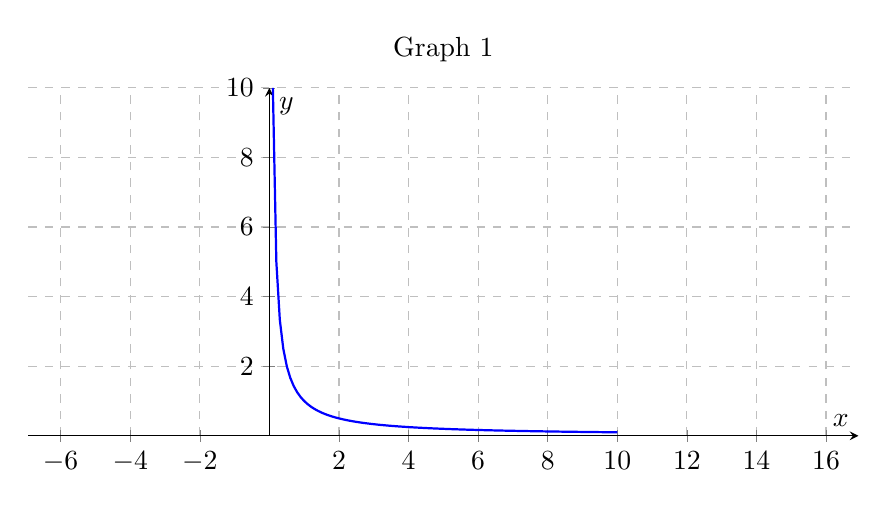
\begin{tikzpicture}
        \begin{axis}[
            domain=0.1:10, % extend the domain to 10
            samples=100,
            xlabel={$x$},
            ylabel={$y$},
            xmin=0, ymin=0,
            xmax=10, ymax=10,
            axis lines=middle,
            legend pos=north east,
            width=\linewidth,
            height=6cm,
            ymajorgrids=true,
            xmajorgrids=true,
            grid style=dashed,
            axis equal,
            title={Graph 1}
            ]
            \addplot[blue, thick] {1/x};
        \end{axis}
    \end{tikzpicture}
    \end{minipage}
    
    &
    
    % Second graph: y = -x^2 + 1
    \begin{minipage}{0.45\textwidth}
    \centering
    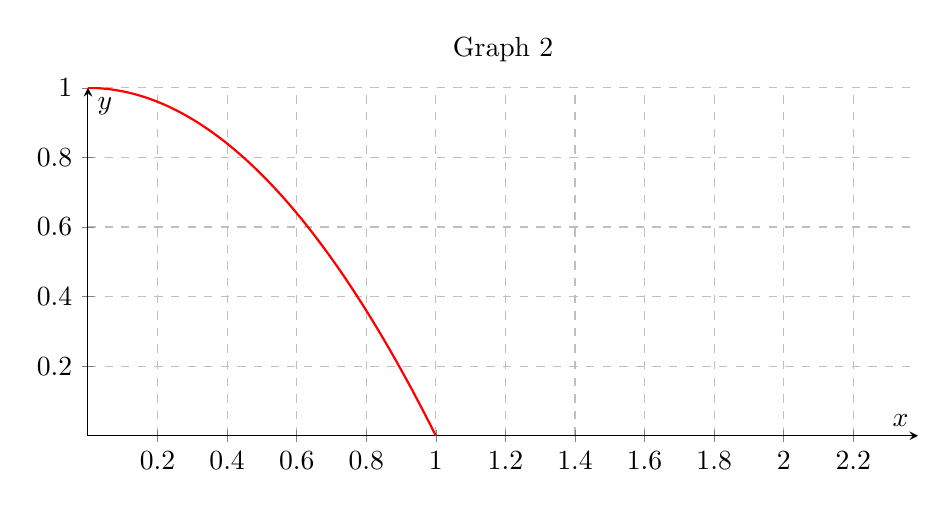
\begin{tikzpicture}
        \begin{axis}[
            domain=0:1, % restrict the domain
            samples=100,
            xlabel={$x$},
            ylabel={$y$},
            xmin=0, ymin=0,
            axis lines=middle,
            legend pos=north east,
            width=\linewidth,
            height=6cm,
            ymajorgrids=true,
            xmajorgrids=true,
            grid style=dashed,
            axis equal,
            title={Graph 2}
            ]
            \addplot[red, thick] {-x^2 + 1};
        \end{axis}
    \end{tikzpicture}

    \end{minipage}
\end{tabular}
Note that in Graph 1, when we increase the number of goods X we need, we progressively need less Y. Conversely for Graph 2, when we need to increase the number of goods for X, we progressively need more and more good of Y. 
\end{document}
